\section{RESEARCH AND TECHNOLOGICAL QUALITY} %8pages
\label{sec:quality}
\subsection{Research and technological quality, including any interdisciplinary and multidisciplinary 
aspects of the proposal}
\label{sec:q1}
Environment models are resources  for enabling robots to perform their
tasks more reliably, efficiently, and competently by using information
about the  environments. The proposed  project \ksem\ (Knowledge-enabled
Semantic Object Maps) investigates a new generation of environment models that
are to enable  robots to perform everyday manipulation  tasks in human
environments effectively and efficiently.   To this end, \ksem\ proposal
extends state-of-the-art  models such  as Semantic Object  Models with
probabilistic  spatio-temporal   information:  they  probabilistically
represent where objects typically are, where objects belong, the state
of  objects  depending  on  their  location  (perishable  objects  are
typically to  be found in  refrigerators), the dependence  of activity
contexts  on  object locations  (if  pots are  on  the  oven then  the
activity   context  is   probably  meal   preparation).   Using  these
representational mechanisms \ksem\ project provides semantic object maps that can
characterize objects and places in the environment with respect to the
role they  play in activities  (affordances). These are  necessary for
autonomous robots to do the right  actions to the right objects in the
right way: when setting the  table, the robot should retrieve the cups
from the cupboard because they  are clean. When cleaning the table the
robot  should  put  the  dirty  cups  into  the  dishwasher  to  clean
them.  Semantic object maps in \ksem\ project  enable the  robot  to  infer  this kind  of  commonsense
knowledge.   Technologically,  \ksem \ will  be realized as  semantic object  models
combined with  relational probabilistic models that  relate objects to
activities, places,  time, roles, etc.  \ksem\ semantic object maps are (semi-)automatically
acquired through the combination of semantic object model acquisition,
the observation of everyday activities, the use of web instructions on
everyday activities and statistical relational learning. Usefulness of 
the \ksem\ project will be demonstrated  in the context of  setting  the  table, 
loading  the  dishwasher and simulating the shopping task (see Figure~\ref{fig:teaser}, and 
our video~\footnote{\url{http://youtu.be/x0Ybod_6ADA}} accepted at AAAI 2011 Video Challenge).
The joint probability distributions of semantic object maps in \ksem are to represent the
dynamic aspects of the environment in the context of everyday
activities, which include:
\begin{itemize}
\item \emph{the typical locations of objects:} cups and plates can
  typically be found on the table, in the dishwasher, and in the
  cupboards;
\item \emph{the home/storage location of objects:} cups and plates are
  stored in a particular cupboard before they are used and after they
  are cleaned;
\item \emph{typical arrangements of objects:} some objects are
  typically used together in certain configurations, for example
  at lunch; %, where we can say which objects belongs where;
  %--- this information can be used then to easy classification
  %and also to find out where a certain object belongs in a given situation;
\item \emph{action-related places}, the places where actions and
  activities are performed;
\item \emph{role/affordance-based object models:} the roles that
  objects play in activities;
\item \emph{time-space-state representations:} the changes of
  objects' state and position over time.
\end{itemize}

\todo{Dejan: SHORTEN}\\
According to the research topics of the \ksem\ project, we will now
briefly review relevant research directions in the areas of semantic
object maps, object perception,knowledge representation for robots, statistical relational models,
spatio-temporal learning, and entity resolution. The project will
explicitly not deal with the research on perception of humans and their activities.
Where needed we will either apply manual labeling techniques or make use 
of the existing frameworks such as e.g. OpenNI~\footnote{\url{http://www.openni.org/}}.
\subsubsection{Semantic Object Maps: Acquisition and Use}
\label{sec:soms}
As semantic object maps include models of the environment structure and the static
components of the environment including the furniture, appliances,
etc. we will first consider the state of the art in the acquisition
and use of 3D semantic object maps for everyday manipulation.

In~\cite{ObjectsOffice}, W\"unstel and Moratz use a graph
representation to detect chairs, but the relation descriptions are
manually estimated, and thus it is unclear whether the proposed method
scales. Posner et al.~\cite{PosnerCumminsNewman08} use probabilistic
graphical models such as Markov random fields to label planar patches
in outdoor urban datasets. Their work is based on that of Anguelov et
al.~\cite{Anguelov05discriminativelearning} and Triebel et
al.~\cite{TriebelAMN07}, which define point-based 3D descriptors and
classify them with respect to object classes such as chairs, tables,
screens, fans, and trash cans in the former, %~\cite{TriebelAMN07},
respectively wires, poles, ground, and scatter in the
latter.%~\cite{Anguelov05discriminativelearning}.

% An EM-based algorithm for learning 3D models of indoor environments is
% presented by Liu et al.~\cite{ThrunEM3D}. The maps are created using
% mobile robots equipped with laser range finders, but they do not
% include any semantic information. Grau~\cite{GrauSceneAnalysis} uses a
% stereoscopic camera system and a knowledge base in the form of a
% semantic net to form 3D models of outdoor environments. A hybrid
% representation including spatial and semantic aspects is proposed by
% Galindo et al.~\cite{GalindoMultiHierarchical} for an indoor
% environment, but their approach needs further investigation.

Iocchi and Pellegrini~\cite{IocchiISPRS}, Mozos et
al.~\cite{MartinezMozos07a}, and Vasudevan et
al.~\cite{vasudevan07cognitive} use 2D laser sensors to create a map
used for navigation and additional semantics are acquired through the
use of vision. An object-based approach for cognitive maps is used to
recognize objects and classify rooms in different categories
in~\cite{vasudevan07cognitive}, while
in~\cite{Mozos2006iros,MartinezMozos07a}, places are semantically
labeled into doorways, kitchens, corridors, rooms.  The advantages of
these representations are straightforward: they keep the computational
cost low enough and base their localization and pose estimation on the
well-known 2D SLAM (Simultaneous Localization and Mapping) problem,
while the problem of place labeling is solved through the usage of
feature descriptors and machine learning.  However, by reducing the
dimensionality of the mapping to 2D, most of the world geometry needed
for manipulation is lost.  Also, the label categories need to be
learned a priori through supervised learning and this makes it unclear
whether these representations scale well.

% With few exceptions, in particular in the area of cognitive
% mapping as \cite{vasudevan07cognitive} and the work of Modayil and Kuipers~\cite{Modayil04}, but also
% including the more recent work by Triebel et al.~\cite{Triebel2007gfki},
% maps do not represent objects relevant to any robot tasks apart from navigation.

For modeling the static part of the environment N\"uchter and
Hetzberg~\cite{nuechter08semanticmaps} classify 3D sensed data from a
laser sensor into walls, floor, ceiling, and doors based on angular
thresholds. Static objects including standing humans are detected
in two steps, first a hypothesis is extracted from a depth image
using an appearance based method, then 3D matching to a model is
performed to evaluate the classification. This however requires 2D
models for all poses of each object to be detected, as well as the
complete 3D models. The same holds true for postures in the case of humans.
Primarily we will base our work on our past work where we have built a
system for autonomous semantic mapping~\cite{mapping11iros}.
\subsubsection{Object Detection, Recognition, and Reconstruction for Pick-and-Place Tasks}
\label{sec:objects}
Semantic object maps in \ksem\ must also include models of the objects of daily use, which
are to be manipulated by the robot. Thus, we now consider recent
work in object detection, categorization, localization, and
reconstruction for robotic object perception.

% A vision-based grasping system which segments objects on a table and constructs
% triangular meshes for them is presented by Richtsfeld and Vincze~\cite{Richtsfeld08}.
% While the presented method is general and works for many objects, it creates
% complex models for certain objects, which could be simplified through the usage
% of geometric primitives. A simplification of the modeling problem is used in
% Grasp-It~\cite{Grasp-It}, where geometric shape primitives are used to model each
% object as a sphere, cylinder, cone or box.

% Geons (geometric icons)~\cite{Geons} can be used to develop generic category
% descriptions using geometric primitives, but also additional category knowledge,
% for the purpose of building libraries of grasp models for a variety of objects.

A computer vision- and machine learning-based method is used by Saxena
et al.~\cite{Saxena08Grasping} to train classifiers that can predict
the grasping points in an image.  This is then applied to images of
unseen objects.  To obtain 3D positions of grasping points, the
authors use stereo cameras, but their approach works reliably only to
the extent provided by the training data.  Another issue is the
segmentation of objects, since grasp points are provided with no
information about what objects are in the scene and to which of them
do the identified points correspond.  Bone et
al.~\cite{Lambert08Grasping} use an accurate line laser and a camera
to build models and identify grasping points for novel objects with
very encouraging results.  However the system was tested only on two
objects, thus its scalability is not clear.

In purely computer vision based approaches, features like the ones described by
Lowe~\cite{lowe04distinctive} or Lepetit and Fua~\cite{lepetit06keypoint} are
used to find matches between parts of a scene and a database of object images.
The problem with these kinds of approaches
is that they only work for objects that are in the database, and since no
knowledge about the 3D information is known, the system can easily make
mistakes and return false positives (e.g., a cereal box containing a picture
of a beer bottle printed on it will get recognized as a bottle of beer).
Some of the solutions adopted involve the offline creation of complete 3D models
for the targeted objects and finding feature spaces to match the partial views
with models in the database, as presented by Collet et al.~\cite{Collet09ICRA}.
Another approach to obtain 3D information directly from camera images is to
project CAD models from a database to the image and search for good matches in
the edges domain, as in Ulrich et al.~\cite{ulrich-etal:09} for example. While
this is a more direct method, it is still dependent on a database of CAD models.

% Available models of complex objects are decomposed into superquadric parts
% by Biegelbauer and Vincze~\cite{SuperQuadrics07} and Zhang et
% al.~\cite{SuperQuadricsAutomotive}, and these models are matched to a point cloud.
% This, however, needs a database of models, and moreover, their decomposition
% into superquadric components, which is often difficult to obtain.
% A sample consensus based approach for model decomposition is presented by
% Schnabel et al.~\cite{Schnabel2007}, where a set of 3D geometric primitives
% (planes, spheres, cylinders, cones and tori) are fit to noisy point clouds.
% Since the point clouds presented there are complete, the authors do not
% need to reconstruct the missing parts.

Thrun and Wegbreit~\cite{Thrun05Symmetries} describe a method for detecting and verifying
symmetries in point clouds obtained from a single viewpoint which works very well for
nicely segmented objects, however the problem of under- or over-segmented objects remains.

Object categorization goes hand in hand with segmentation and is usually
performed using a single sensing device.  Given a large set of training
values containing all possible views, most approaches try to abstract the
problem by using features like the ones proposed by Quack et al.~\cite{quack2007emf},
Yan et al.~\cite{yan2007mbo}, and Savarese and Fei-Fei~\cite{savarese2007goc},
which work best on low scale and texture variance.  The
scaling variance can be reduced significantly by a previous segmentation.
% Saxena et al.~\cite{saxena:07:iccv} try to extract the 3D world out of only one view in
% order to improve the segmentation of objects.  Another approach is to
% actively explore the environment and segment objects using the motion to
% generate 3D shape information, as done by Welke et al.~\cite{welke2008osu}
% and Feldman and Weinshall~\cite{feldman2008msa} for example.

To improve the segmentation, Lai and Fox \cite{Lai-RSS-09} take a randomized approach
by classifying a ``soup of segments'' generated by different combinations of clusters,
and use the results to get a final segmentation. They also explore different domain
adaptation techniques in order to incorporate synthetic data in training their classifier.
Though they are working with outdoor data, the same techniques can be applied to segment
and classify indoor objects using low resolution 3D data, e.g. from time-of flight cameras.
Our starting point will be however our past work on object categorization and recognition
as presented in~\cite{marton11ijrr}.
\subsubsection{Symbolic Knowledge for \ksem}
\label{sec:knowledge-representation}
For performing high-level tasks, robots need large amounts of semantic information from their environment model,
like the types, locations and properties of objects. Very few systems exist that offer this kind
of deep semantic environment information.

At the highest level of abstraction, one considers
the recognized objects, whose semantic meaning is only implicitly represented: Humans immediately
associate various properties with something called a ``cupboard'', while robots usually do not have
this kind of knowledge. Without an explicit knowledge representation, different robots or even different
parts of the same robot may have a very different notion of an object.

Deeper semantic representations, which also describe object properties, such as the point at which to grasp
an object or location of the opening of a container like a bottle, are used by Okada et al.~\cite{okada2007iros} but are mainly hand-coded
and do not leverage the power of hierarchical, abstract knowledge representations.
Galindo et al.~\cite{galindo08taskplanning} present a system for automatically building maps that
combine a \emph{spatial hierarchy} of local metric and global topological maps with a \emph{conceptual
hierarchy} that describes some semantic properties of rooms and objects. In this respect, their approach is
similar to ours, but the conceptual hierarchy is much simpler and the spatial description much coarser.\\
In~\cite{iros10kcopman} we developed a system that generates symbolic representations
of perceived objects and scenes and infers answers to complex queries that require the combination of perception and knowledge
processing.

\subsubsection{Statistical Relational Models}
\label{sec:markov}

In order to declaratively represent highly complex domains, in which there are relations between a variable
number of relevant entities and which are furthermore governed by uncertainty, one requires a representation
formalism that combines statistical with relational components, abstracting away from concrete entities
to compactly represent general principles about the relevant aspects of the real world.
In statistical relational learning, a number of such formalisms have been proposed,
as presented by Getoor and Taskar~\cite{getoor07introduction} and De Raedt~\cite{DeRaedt08Learning}.
Statistical relational learning methods have countless applications, including collective classification~\cite{neville03collective},
link prediction~\cite{taskar03link} and object identification~\cite{singla06entity}.
In particular, the methods of statistical relational learning allow
to represent full-joint distributions over logical propositions about a changing set of entities in
a concise, declarative manner, and they provide a fully integrated framework for learning and inference. Therefore,
they are ideally suited to the representation of the probabilistic components of semantic object maps in \ksem as we envision them,
since we need to consider, for example, spatial relations between objects in the environment, their attributes
changing over time, their relevance to activities taking place and the effect these activities may have upon them.

\subsubsection{Spatio-Temporal Learning}
\label{sec:spatio-temporal-learning}

Our intended research in learning spatio-temporal structures for
semantic object maps in \ksem is inspired by research in visual analytics for the analysis
of movement data. Andrienko et al. learn concepts like the
working place, the living place, typical navigation routes and other
spatio-temporal behavior patterns from GPS-data from their car
\cite{Andrienko07}. While in their case, the data mining tasks are
performed by human experts using visual analytics methods, other
researchers such as Liao et al.\ \cite{Liao07a,Liao07b} perform some
of these learning tasks using probabilistic learning
methods (hierarchical conditional random fields).
Acquiring such models is also investigated in the pervasive
systems community, where Philipose and his colleagues
\cite{Pentney07,Landwehr07} and Intille and his research group
\cite{Intille06} learn models of daily activities from ubiquitous
sensor networks.

% If maps are to be used for more than navigation and mere obstacle avoidance,
% a semantic interpretation of the observed scenes is required, which
% necessitates a meaningful labeling of objects appearing in mapped scenes.
% Posner et al.~\cite{PosnerCumminsNewman08} propose a two-stage process to
% solve this problem, where, at the local level, classification is based on
% appearance descriptors, and at the global scene level, Markov random fields
% (MRFs) are applied to model relationships.  Triebel et al.~\cite{Triebel06robust3d}
% draw upon statistical relational learning methods, specifically
% associative Markov networks, to solve a similar problem --- again, however,
% on laser data only and at a low level of abstraction.

%\fbox{Include the trajectory learning work from \cite{stulp09compact}?}
%\fbox{Zoltan: maybe in prev work of the proposers, right? here maybe their related work}

\subsubsection{Entity Resolution}
\label{sec:entity-resolution}

A key problem that has not yet received substantial attention in
autonomous robotics is the inference about whether two different
observations resulted from the same real world object. This type
of inference is needed to recognize previously observed objects again,
which in turn must be solved to build spatio-temporal environment models.

% This problem can be viewed as an entity resolution problem that arises
% in many information integration scenarios: Given two or more sources
% containing records on the same set of real-world entities (e.g. mapped
% objects), the problem is to determine which of the records actually
% refer to the same object, as we typically have no unique identifiers
% that tell us what records from one source correspond to those in the
% other sources. Furthermore, the records representing the same entity
% may have differing or even partially contradictory information.  For
% example, one record may have an attribute falsely assigned (as a
% result of sensor inaccuracy), another may be missing some fields. An
% entity resolution algorithm attempts to identify the matching records
% from multiple sources (i.e. those corresponding to the same real-world
% entity), and merges the matching records as best as it can. Entity
% resolution algorithms typically rely on user-defined functions that
% (a) compare fields or records to determine if they match (are likely
% to represent the same real world entity), and (b) merge matching
% records into one, and in the process perhaps combine fields (e.g.,
% creating a new name based on two slightly different versions of the
% name).

While early work has often phrased the problem as a
classification problem where a pair of records would be independently
classified as either ``matching'' or ``non-matching'' \cite{fellegi69linkage}, % note: no need to mention authors here
more recent approaches have
phrased the problem as link prediction in statistical relational
models, e.g. Singla and Domingos~\cite{singla06entity}: One defines an
equivalence relation over entities and considers, in a probabilistic
setting, any predicates that state the same things about two entities
as evidence for the entities referring to one and the same real-world
entity; the importance of certain predicates can be learned from
statistical data.  Most importantly, this relational approach
considers the objects collectively and does not assume that the
equivalence of a pair of objects is independent of other
equivalences. \\
%Intro to the proposal, Semantic maps (temporal and spatial aspects), multidisciplinarity vs interdisciplinarity:
%robotic perception (2D + 3D), AI and machine learning
\subsection{Appropriateness of research methodology and approach}
\label{sec:q2}
In order to clarify the motivation from above, we identified
the following three subgoals of the project: \\
\textbf{Subgoal 1: Representations in \ksem} will be hybrid by
  integrating geometric descriptions (such as primitives, meshes,
  voxels), first-order description-logic-based symbolic representations
  (e.g. symbolic object properties, relations between objects and object
  classes) and probablistic first-order representations (including
  Markiv logic and Bayesian logic networks).
  Together with a representation language based on OWL (Web Ontology
  Language) and a concept ontology based on researchCyc (an encyclopedic
  knowledge base), these representations can be stored, extended and
  they can be queried by a Prolog-based inference mechanism.\\
\textbf{Subgoal 2: Perceptual mechanisms} for detection,
  categorization, recognition, localization and reconstruction of
  objects of daily use. Additionally, the robot needs capabilities to
  perceive and interpret arrangements of objects (spatially and/or
  temporally related). This includes methods for identity resolution and
  estimation of object state based on partial information and context to
  allow affordance-based manipulation. \\
\textbf{Subgoal 3: Learning of semantic object maps} for autonomous world state
  interpretation. Some of the identified learning problems are:
  \begin{itemize}
    \item Learning typical locations of objects such as storage or
      usage locations, and interpretation of containers based on a
      generalization of their contents (e.g. fridge);
    \item Learning action-related places are places where actions are
      performed or objects take on certain roles in actions. This allows
      a robot to learn e.g. the concept of a chair by its role to
      support people as opposed to purely geometric or appearance
      based recognition;
    \item Learning arrangements of objects is important to abstract from
      a continuous coordinate system of object locations to a symbolic,
      relational model of a scene which allows e.g. for context
      interpretation of a table arrangement;
    \item Knowledge-intensive learning from selected web sites such as
      researchCyc for encyclopedic knowledge, ehow.com or wikihow.com
      for task instructions and the OpenMind Indoor Common Sense (OMICS)
      knowledge base. This constitutes important background information
      for \ksem\ project.
  \end{itemize}
  These learning problems require autonomous and on-demand (partial) 
  processing of sensor data to enable life-long learning.\\
% \textbf{Subgoal 4: Applications for robot control} to enable
%   real-world problem-solving within a household assistance system such
%   as execution of everyday manipulation actions (e.g. emptying a
%   shopping bag, set the table for a given meal, or cleaning the table,
%   while stowing items in their respective places, such as the fridge or
%   dish washer) and task-dependent partial environment mapping.
\begin{figure}
  \begin{centering}
    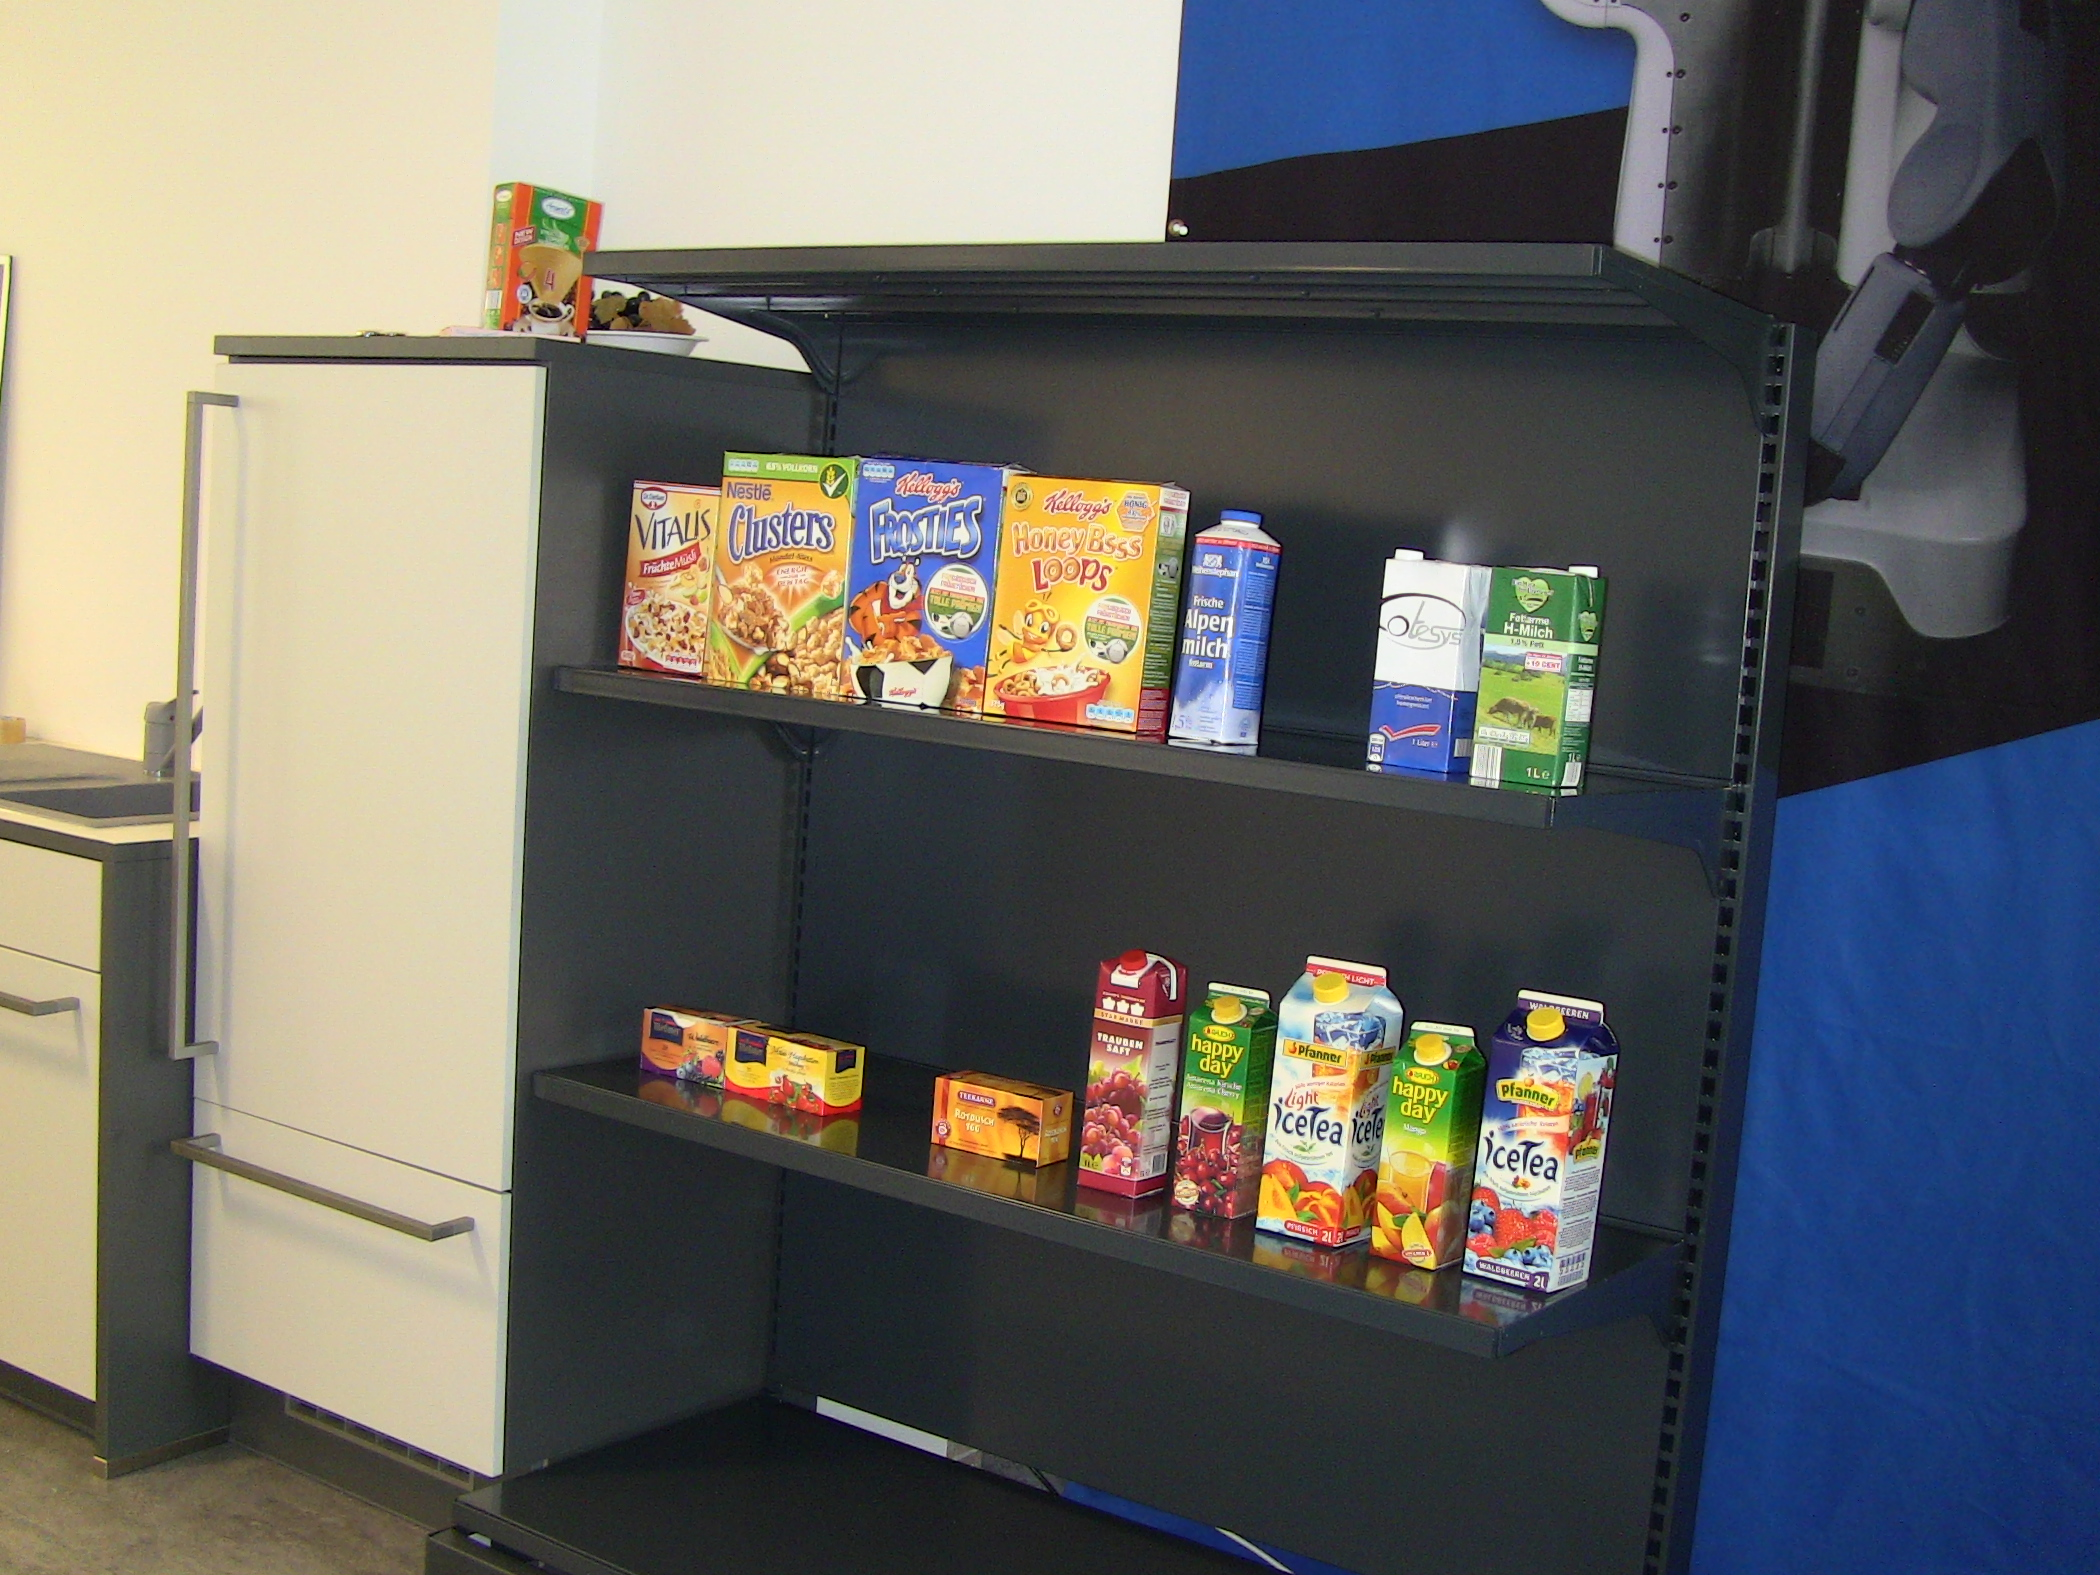
\includegraphics[width=0.3\textwidth]
    {figures/storage_rack.JPG}
    {\large$\rightarrow$}
    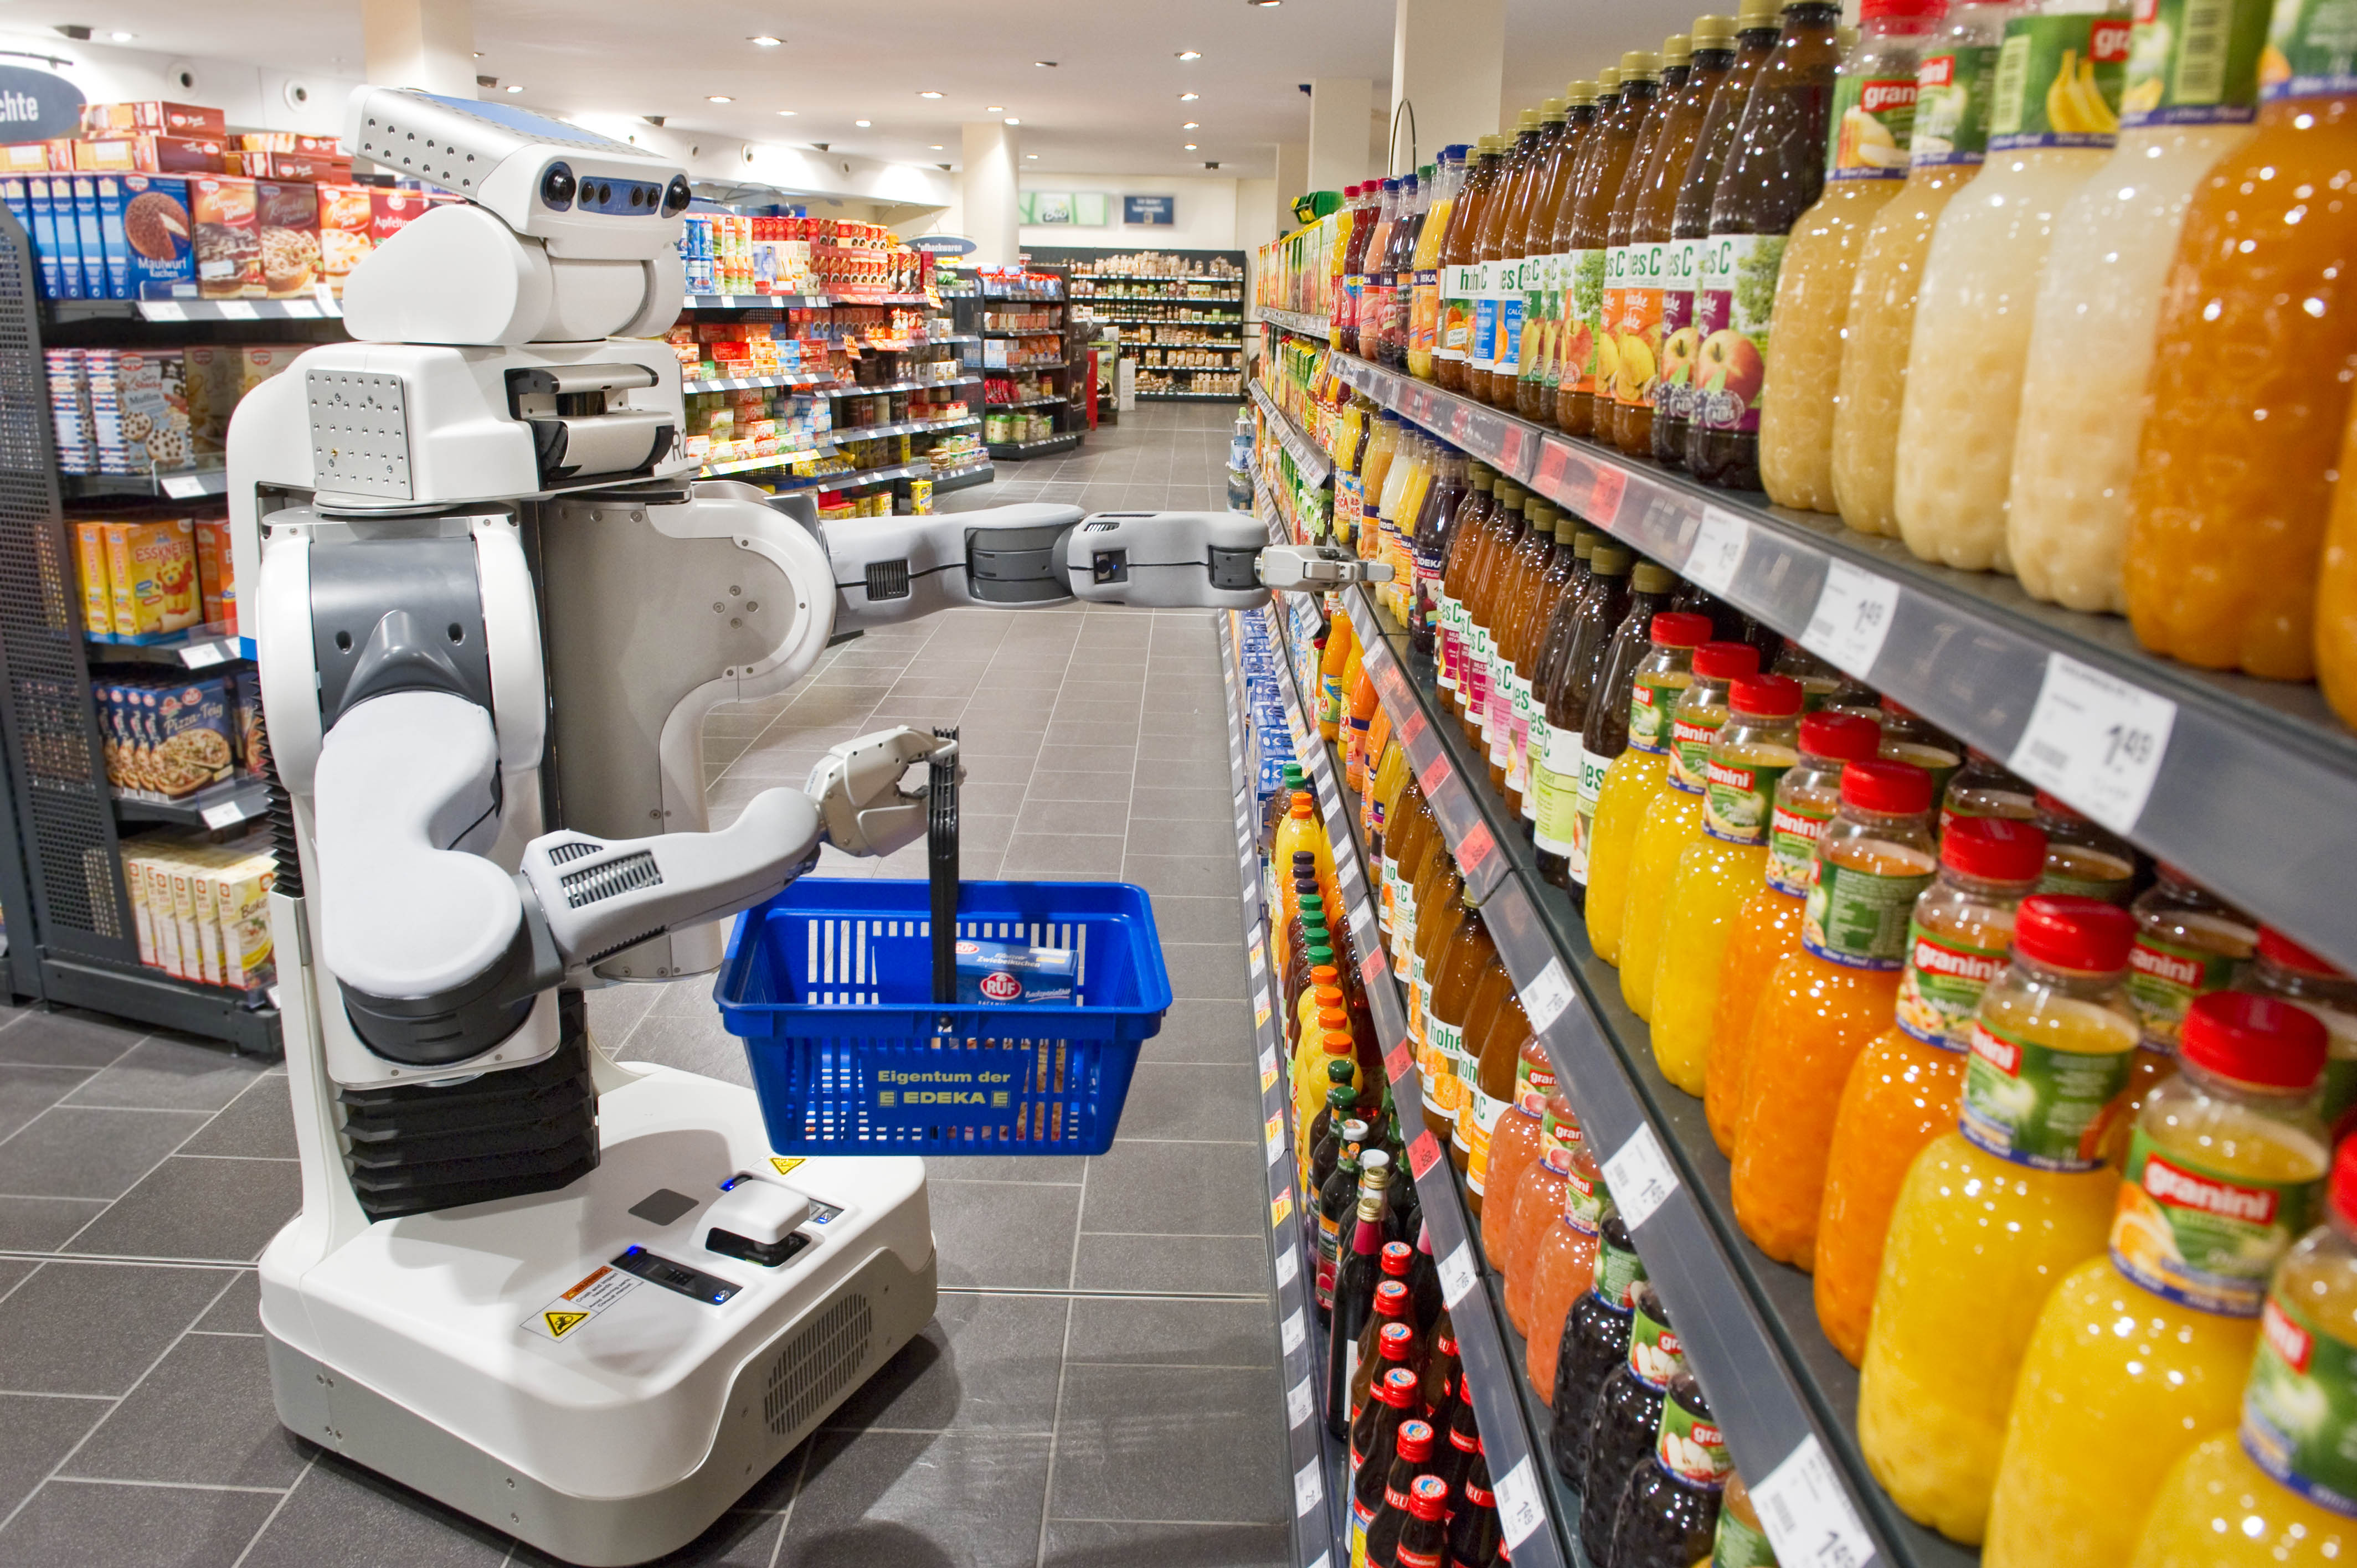
\includegraphics[width=0.3\textwidth]
    {figures/pr2_edeka_basket_1.jpg}
    {\large$\rightarrow$}
    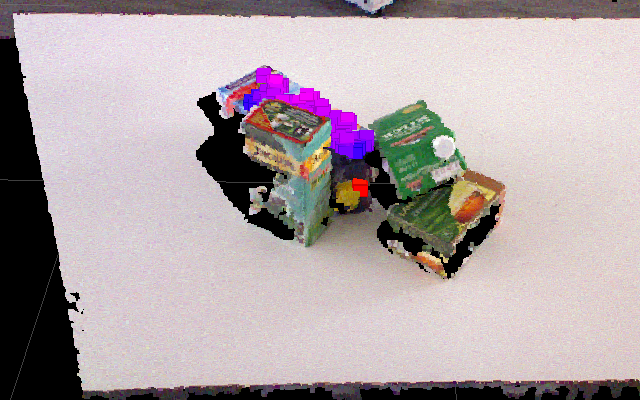
\includegraphics[width=0.3\textwidth]
    {figures/clutter-objects.png} \\
    % {\large$\rightarrow$}
    % \includegraphics[width=0.3\textwidth]
    % {mapping/clutter/basket_flipped.jpg}\\
    \vspace{2ex}
    
\includegraphics[width=0.3\textwidth]
    {figures/all_segmented.png}
    {\large$\rightarrow$}
    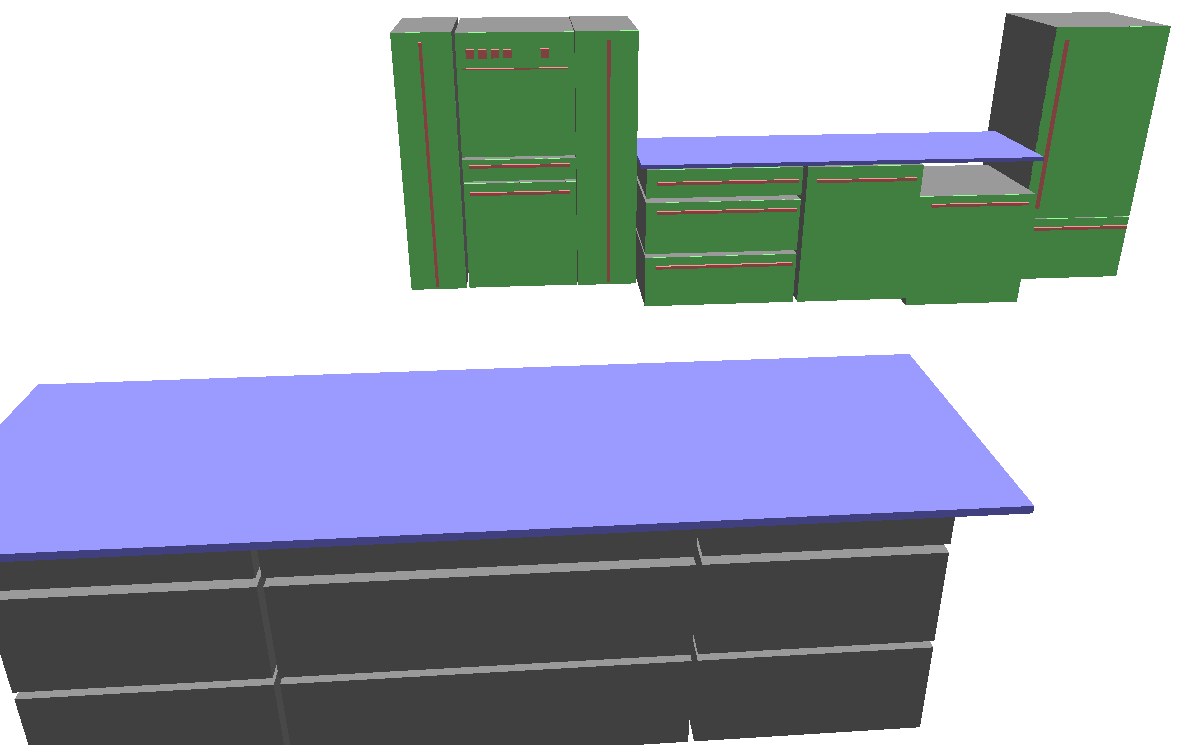
\includegraphics[width=0.3\textwidth]{figures/xml_map.png}
    {\large$\rightarrow$}
    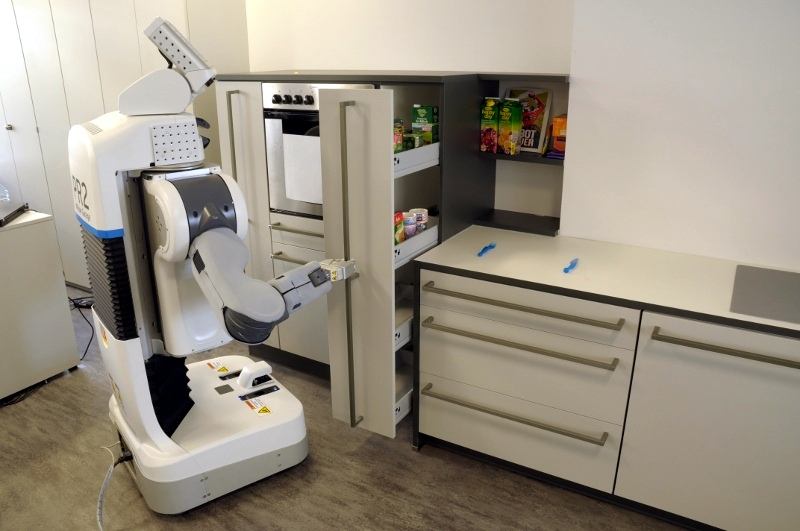
\includegraphics[width=0.3\textwidth]
    {figures/pr2_highdrawer.jpg}
  \end{centering}
  \caption{Robot simulating a shopping task and making use of \ksem\ generated semantic object map. \textbf{Top-left, top-middle:} 
    typical objects and scenes that robot is to perceive and manipulate using mechanisms from \ksem. 
    \textbf{Top-right:} recognition and pose detection of objects in cluttered scenes. \textbf{Bottom-left, bottom-middle:} 
  3D-based environment reconstruction and static world modeling. \textbf{Bottom-right:} Robot learns typical storage locations
using e.g. WUP similarities and places the object where it belongs to.}
  \label{fig:teaser}
\end{figure}
All of the subgoals named above are to be implemented in a system that
is to run on real robot platforms in real household environments.

The project's goals will be achieved in three work packages, reflecting
the previously identified subgoals.

\subsubsection{Work Package 1 (WP1) : Representations of \ksem\ semantic object maps}
\label{sec:wp1}
The first work package is concerned with achieving subgoal 1, the design
and implementation of appropriate representational and reasoning
mechanisms required by \ksem. It is subdivided into the following
three tasks.

\begin{description}
  \item[Task 1.1: OWL Concept Taxonomy] The basic symbolic
    representation will be realized using SWI Prolog with an additional
    package for OWL (Web Ontology Language). Based on previous work of
    the return host, we will specify concepts for objects, object groups,
    places, object and scene states, and we will anchor these concepts
    in the data structures used for map representation and those
    generated by the perception routines to be developed in WP 2.
    As an example, objects of daily use will have locations attached to
    them, such as \emph{home} places, state-dependant locations (dish
    washer when dirty), and locations where they belong (e.g. within
    arrangements of objects on a table).
  \item[Task 1.2: Spatial Relations and Scene Representation and
    Reasoning] Representational primitives of key importance in
    \ksem\ project are qualitative as well as quantitative spatial relations.
    They are essential for parameterizing robot actions and
    communicating abstract information about the environment,
    respectively. While quantitative relations can be obtained in a
    straight-forward manner, qualitative will be realized following an
    approach inspired by~\cite{Gapp95} and will be learned from
    observations of human activity.
    
  \item[Task 1.3: Representations of Action-related Concepts]
    In order to relate objects, scenes, etc. to the actions and the
    activities they are involved in, we will develop \emph{action-related
    concepts} as our key representational mechanisms. Preliminary
    investigations in this regard have been performed in the context
    of mobile pick-and-place tasks, where the return host group has
    developed the notion of \emph{action-related places} (\textsc{ARPlaces}), i.e. the
    set of robot poses from which a given pick task is predicted to be
    successful. A second starting point is our previous work on
    \emph{grounded action models} (\textsc{GrAM}), where we have introduced a
    new class of concepts in description-logic-based knowledge
    representations, integrating actions and action models into the
    knowledge representation and inference mechanisms of intelligent
    systems. 
     
  % \item[Task 1.4: First-order Probabilistic Representations of
  %   \ksem\ semantic maps] In previous work, we have developed \textsc{ProbCog}, 
  %   a statistical relational learning system that supports efficient
  %   learning and inference in relational domains, focusing mainly on
  %   probabilistic logical models. Based on a common data model, we
  %   integrate various representation formalisms and have successfully
  %   extended the expressiveness and practical applicability of existing
  %   approaches. \textsc{ProbCog} thus provides a coherent probabilistic framework
  %   that enables robots to deal with a high degree of uncertainty and
  %   complexity in a variety of application contexts, including adaptive
  %   plan generation for under-specified tasks and heuristic generation.

  %   This work package will extend \textsc{ProbCog} with mechanisms needed
  %   for spatial, temporal and spatio-temporal reasoning. Using these
  %   extensions. we will be able to probabilistically learn and reason about
  %   the spatial and temporal aspects of \astom s.

  %   One necessary extension is the inclusion of continuous variables,
  %   which are needed to represent coordinates and quantitative
  %   restrictions on coordinates. One of the key research questions here is
  %   to find suitable representations without blowing up the size of the
  %   graphical models representing the respective joint distributions.
\end{description}

\subsubsection{Work Package 2 (WP2): Perception}
\label{sec:wp2}
The objective in WP~2 is to achieve subgoal 2, i.e. achieving the
perceptual capabilities required for object and scene recognition and
interpretation, object detection and reconstruction. 
\begin{description}
\item[Task 2.1: Object Detection and Perception] In this task, we will
  design, implement and analyze a perception system that enables
  the robot to infer \emph{when} \emph{which} object is \emph{where} by
  accomplishing the following perceptual task: given (1)~a set of
  perceptually distinct object instances (e.g. textured mugs, cereal boxes), 
  (2)~a set of perceptually indistinguishable object instances
  (e.g. plates, bowls) and (3)~a set of regions of interest (e.g. tabletops, counters),
  detect and localize these objects of interest whenever they are present in those regions.
  The result is a set of time-stamped observations that
  include the object of interest, its pose, and the respective region of
  interest.

  The research in this work package focuses mainly on object identity resolution 
  and the inference about whether objects have been removed from regions of interest.
  Object identity resolution is the problem of deciding whether or not two partial views
  of some objects in the environment taken at different times $t_1$ and
  $t_2$ refer to the same object in the environment. The aspects of the problem
  that render this inference task hard are that the different views potentially have
  little overlap, that the views are corrupted by sensor
  noise and specular reflections and that views might be limited
  through occlusions. We will investigate how we can apply and adapt
  mechanisms from entity resolution originally developed in the area of data
  mining to better handle the spatial and temporal context
  of this perception task~\cite{Blodow10Humanoids}.
\item[Task 2.2: Scene Perception, Interpretation and Analysis]
  This task will investigate the knowledge-based perception
  mechanisms for scenes and object arrangements. The inclusion of
  knowledge-based mechanisms will enable us to improve scene perception
  through the use of prior knowledge, the semantic object model of the
  environment, knowledge about everyday activities, and the effects of
  everyday activities on the situations in the environment. WUP similarities
  that explore the relatedness among an ontology of objects will be explored
  at first~\cite{wup}.
\item[Task 2.3: Perceiving Object States]
  In the project \ksem, the real-world perception of object states is
  beyond the scope of the project, but we still need to realize
  perception mechanisms for state estimation in order to realize a
  complete and integrated system.

  We will simplify the state estimation in two ways. First, we will use
  --- where-ever possible --- sensor-equipped objects in distributed sensor
  networks that can estimate their own states, e.g. whether they are
  filled.
  Second, for those states that are needed but cannot be perceived
  otherwise, we will simplify the perception tasks by making the states
  perceptually distinctive, e.g. by using RFID tags to store state
  information or by color coding states.
\end{description}

\subsubsection{Work Package (WP 3): Acquisition and Learning of \ksem\ semantic object maps}
\label{sec:wp3}
In this work package, we focus on the learning problems in 
\ksem\ which can be described as follows: \emph{Given} (1)~background
knowledge needed for learning of semantic object maps,  and (2)~a stream
of time-stamped partial observations of situations concerning what is
on tables, on the counter, the states of objects, and object
arrangements, \emph{learn} a mapping for this particular environment.
\begin{description}
\item[Task 3.1: Learning Grounded Representations] The
  type of information that we want to leverage here comes from web instructions.
  To make sense of web instructions, one first needs to apply natural language
  processing techniques. By using a parser based on probabilistic
  context-free grammars (PCFGs),
  return host group has showed how to obtain the structure of sentences and was able to assign to each word an appropriate synonym ring.
  They then used the WordNet lexical database in order to disambiguate word senses based on learned
  correlations between entity types, action verbs and prepositions, and to furthermore
  link the actions and entities appearing in instructions to concepts within the Cyc
  upper ontology. In this way, they can semantically interpret the set of instructions that
  constitutes a particular activity, which opens up 
  new possibilities for detecting these activities within the environment.

\item[Task 3.2: Learning Important Locations] 
  Key locations where certain actions take place need to be identified from
  observation data, both for the learning of action-related places
  and the understanding of human behavior. To this effect, we will need to develop extensions
  to existing methods such as hierarchical conditional random fields
  that also take related actions into account.

  Additionally, the typical and storage locations for objects have to
  be inferred from the probabilistic models built by observations and
  web instructions.
  An important aspect to consider is that \ksem\ needs to learn the distributions
  of locations both for (1)~\underline{specific objects} and (2)~objects of a
  \underline{specific type}.

\item[Task 3.3: Learning Object Arrangements]
  We are planning to expand the perception and learning system we developed
  to consider spatial relations between different objects just as it considered relations between
  different parts of objects. We will be using \emph{WUP} similarities.
  An example of such a feature is a qualitative spatial relation
  such as \emph{left of}, which is represented as a 
  pair of positions $\langle$ \emph{o,refo} $\rangle$ where
  \emph{o} is the position of an object and
  \emph{refo} is the position of the reference object. So
  \emph{P(left-of(o,refo))} denotes the probability that with
  respect to their coordinates the object \emph{o} would be
  considered to be to the \emph{left of} the object \emph{refo}.

  It is also important to note that qualitative spatial relations
  depend on the object types. Depending on whether the
  object pair would be a plate and a fork or a building and a gate,
  the expected positions satisfying the relation would be very
  different. We intend to learn appropriate probability distributions
  from observations of human activities.

\item[Task 3.4: Lifelong \ksem\ Learning]
  In this task, we will realize a 
  \emph{Passive Perception} system, i.e. a set of mechanisms that enable the robot to 
  remember scenes that it encounters while performing its activities, storing them 
  as memory structures in the knowledge base for incremental learning. In that sense we will implement fast 
  logging mechanisms for raw and partially processed sensor data, derive
  sophisticated memory infrastructure formats (aka time-stamped objects store) 
  and develop interfaces for continuous and on-demand processing of previously observed data.
\end{description}
%kinect, mechanical turk, pcl, RGBD slam, hand-held devices, google cloud robotics, semantic vision challenge, 
%aim at the realistic and grounded application + demo
\subsection{Originality and Innovative nature of the project, and relationship to the state-of-the-art of 
research in the field}
%An integrated approach, no AI and classification methods, man-in-the-loop (mechanical turk), Knowrob
The ultimate goal of the project \ksem\ is the investigation of 
environment models that can be inferred from a combination of 
environment exploration and activity observation. To this end, we 
will design, implement and empirically analyze semantic model 
acquisition mechanisms for objects and everyday activities in order 
to generate semantic object maps of human living environment.


As an example, consider the following query that might arise within a
household scenario: A human asks the robot to retrieve a glass he had
been drinking from earlier. This simple request can spawn several queries to
\ksem\ system, such as: Where is a glass that this person had contact with earlier?
There might be multiple glasses, so the system has to select the one
which was used for drinking and disregard other glasses that the human
might have cleaned earlier. Also, for picking up the glass, grasp
analysis might need a surface mesh of the object or a precomputed list
of applicable grasps, and the motion planner needs an occupancy voxel
map or surface mesh of the whole environment for collision avoidance or
possibly additional manipulation constraints linked to the glass, such
as maintaining a vertical orientation over the whole action.
A system that is able to tackle above described challenges, to the best of our
knowledge, does not exist.\\
The system will gain the maximum leverage from the algorithms and code available
in Robot Operating System~\footnote{\url{www.ros.org}} as well as from the cooperation
with the world renowned scientists involved in the PR2 Beta Program~\footnote{\url{http://www.willowgarage.com/pages/pr2/pr2-community}}.
In particular we plan to collaborate with and search expertise from Rachid Alami from LAAS, Wolfram Burgard
from University of Freiburg, Ben Pitzer from Bosch RTC, Brian Gerkey et al from Willow Garage Inc, 
Kei Okada from University of Tokyo, Herman  Bruyninckx from Katholieke Universiteit Leuven and Maxim Likhachev 
(previously University of Pennsylvania, now Carnegie Mellon University).
All enlisted scientists have been consulted and confirmed their participation.
\subsection{Timeliness and relevance of the project}
With all the recent advances in the field of personal robotics and with first
personal robots projected to be deployed in households within next 5 to 10 years, 
\ksem's relevance is enormous for robots to perform in highly dynamic and unpredicted
situations. It will also enable researchers from other fields such as artificial intelligence, 
psychology, ergonomy, etc to get a grasp at the data and study human living patterns, 
social acceptance of robots and other high-level concepts.
The \ksem\ project's relevance under the Marie Curie fellowship within a European 
setting is connected to the innovative ideas it introduces by combining in a novel way 
approaches to build semantic environment models to be used in robots' everyday operations.
The applicant will need to be additionally trained within the host groups, as will be discussed in Section 
\ref{sec:training}, to pursue the proposed research, which is also a significant part of the Marie Curie program.
Since the \ksem\ project is setup such to exploit the mutual leverage with the open source ROS 
community and the PR2 Beta community 
in terms of code re-usability, feedback from other experienced researchers and critical reviews, 
it will make a significant contribution in enhancing the continuously advancing scientific excellence within Europe. 
Both the applicant and the  environment in which the project will be realized will benefit significantly from the 
realization of the proposed project, since also members, senior and junior ones, from the 
host group will have their opportunity to assist the \ksem\ research. \\
%It will help specify environments for Robots and thus accelerate bringing of robots into peoples' homes
%Point out examples such as openCV, PCL, gmappping, KnowRob, etc

\subsection{Host research expertise in the field and quality of the group/supervisors}
Michael Beetz from Intelligent Autonomous Systems (in continuation IAS) group, Technische Universit\"at 
M\"unchen (TUM) will represent the return host organization in the project and Pieter Abbeel and Ken
Goldberg, University of California at Berkeley (in continuation Berkeley) will represent
the outgoing host organization. 
Prof. Beetz is a vice coordinator of the German national cluster of excellence 
COTESYS (Cognition for Technical Systems) where he is also co-coordinator of the research area 
``Knowledge and Learning''. 
%Prof Beetz was a member of the steering committee of the European 
%network of excellence in AI planning (PLANET) and coordinating the research area ``robot planning''. 
%He is associate editor of the AI Journal. 
His research interests include plan-based control of 
robotic agents, knowledge processing and representation for robots, integrated robot learning, and cognitive perception.
Prof. Beetz has published over 200 articles in the first-class conferences and
journals in the fields of robotics, computer vision and artificial 
intelligence~\footnote{http://ias.cs.tum.edu/publications}.
Currently he is leading a group of 2 postdoctoral fellows, 25 grad students and a large number
of undergrad students and visiting researchers. He is also serving as a principal investigator 
for TUM's PR2 Beta Program. Prof. Beetz has successfully coordinated and trained 
more than 15 postdoctoral fellows and PhD students, in addition to a larger number of 
master's and diploma students. Most of his group alumni currently hold faculty positions in 
Universities and Research Institutions in Europe and United States.
The equipment that is required for the realization of the project at the host organization is already available. In
particular, three robot manipulation platforms -- a PR2\footnote{\url{http://www.willowgarage.com/pages/pr2}}, an
iCub\footnote{\url{http://www.robotcub.org}} and a custom-built robot
with KUKA lightweight arms and DLR/HIT hands -- are available for
real-world experiments on a daily basis. So is the testbed kitchen environment with an ample
set of ubiquitous devices such as Kinect sensors, ceiling cameras, RFID readers, etc.\\
%Michael: planning, knowledge for robots, 3D perception, mobile manipulation, Pieter and Ken: machine learning, 
%mobile manipulation, reinforcement learning
Pieter Abbeel's research interests lie at the intersection of robotics, machine learning and control. Current
projects focus on the application areas of personal robotics, surgical robotics and autonomous flight.
In the personal robotics arena, thus far Abbeel's group's focus has been on the manipulation of deformable
objects---with the particular challenge application of fully autonomously performing laundry. They
enabled WillowGarage's PR2 robot to successfully fold 50/50 previously unseen towels. Abbeel's group
has also resurrected the Berkeley Surgical Robots with the aim of automating selected surgical skills.
In his thesis work, Abbeel has developed apprenticeship learning algorithms, which leverage expert
demonstrations to teach a robot to perform certain tasks. These apprenticeship learning algorithms enabled
a quadruped robot to climb across rocky terrains, and they resulted in by far the most capable autonomous
helicopter to-date. In particular, this work resulted in the first autonomous completion of a wide variety of
maneuvers, including in-place flips, in-place rolls, loops, hurricane, knife-edge, and even auto-rotation
landings, tic-tocs and chaos, maneuver only exceptional human pilots are able to perform. Currently
Abbeel's group is investigating extensions thereof with application to robotic manipulation.

Goldberg received his PhD in Computer Science from CMU in 1990 and studied at the University of
Pennsylvania, Edinburgh University, and the Technion. From 1991-95 he taught at the University of
Southern California, and in Fall 2000 was visiting faculty at MIT Media Lab. Goldberg and his students
work in two areas: Geometric Algorithms for Automation, and Networked Robots. In the first category, he
develops algorithms for feeding, sorting, and fixturing industrial parts, with an emphasis on mathematically
rigorous solutions that require a minimum of sensing and actuation so as to reduce costs and increase
reliability. In the area of Networked Robots, Goldberg and colleagues developed the first robot publically
operable via the Internet (in 1994). He has published over 100 research papers and edited four books. In
2004, Goldberg co-founded the IEEE Transactions on Automation Science and Engineering and is
Founding Chair of its Advisory Board. Goldberg was named National Science Foundation Young
Investigator in 1994 and NSF/Whitehouse Presidential Faculty Fellow in 1995. He is the recipient of the
Joseph Engelberger Award (2000), the IEEE Major Educational Innovation Award (2001) and was elected
IEEE Fellow in 2005.

\begin{footnotesize}
\begin{multicols}{2}
\bibliography{ksem}
\end{multicols}
\end{footnotesize}
\newpage